\chapter{Testing the installation}
\section{Introduction to testing}
Testing is an important part of the project. It is a great opportunity to get an impression of how the visitors of the library experience the installation.

%When performing a test, one should be humble and consider all feedback valuable.

The testing of the installation took place at Hj{\o}rring Library during its opening hours in December. The goal was to see how people interacted with the installation and whether they grasped the concept. The focus for the project is to entertain people of all ages, so it is interesting to get an overview of how this goal is achieved. It was also of great importance to observe if the installation actually drew visitor's attention, or if people just walked past it without noticing it. It was of interest to see if any patterns or tendencies emerged.

\subsection{Observations}
The test was conducted as a bipartite test. The first part of the test focused on the visitors, while the second part focused on the installation itself.\\
During the first test, one group member focused on monitoring people's habits, gender and ages, while the other group member interviewed the visitors. The second test was a user test where the tracking of people was in focus.

For the purpose of the test, two types of visitors were defined: active users and passive users. An active user is a visitor that by own initiative chooses to engage with the installation. A passive user is defined as a visitor that casually walks past the installation without deciding to engage with it further.

Two group members were present at the installation to observe people walking by. It was important that the group members did not position themselves too close to the installation, so that they would have an influence on the way people reacted. One of the group members focused on people using the installation actively and the other group member focused on people using the installation on a passive level.\\

\subsection{Interviews}
The testers were positioned on either side of the installation, to ask people who walked by the installation to participate in answering some simple questions. People were kindly asked if they were interested in giving some feedback to improve the user experience.

The idea of placing two members on either side of the installation was in order to gather information after the visitors had the chance to engage with the installation. The questionnaire prepared for the interviews is illustration on figure \eqref{fig:test_interview} and it contained the following questions:

\begin{figure}[H] 
\centering 
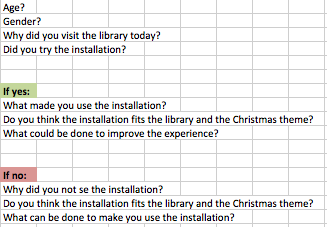
\includegraphics[width=0.75\textwidth]{Pictures/Test/Interview.png} 
\caption{Figure showing the questionnaire used for the interview} 
\label{fig:test_interview} 
\end{figure}

\subsection{Testing the installation}
The second task of the testing was to run a user test which main focus was to evaluate the installation at the library. One of the primary aspect of the installation is the possibility to track several people at once. Therefore it was of great importance that the program works as intended.\\
The test was primarily concentrated on tracking people and applying the BLOB analysis. The following tests were conducted: 
\begin{itemize}
\item Fidelity test
\item Number of simultaneous tracking
\end{itemize}

\section{Results}
After going to Hj{\o}rring Library to run the different tests, the analyzing part was to be made. The testing ran for an entire day, to see if there were any changes in tendencies during the day. The testing will be evaluated and analyzed in the following subsections.\\
All test participants were offered some Christmas treats in return for the help. In addition the majority of visitors were positive and friendly-minded. Unfortunately, December is a busy month, so many people were occupied and did not have time to participate in the testing. On the day of testing there was a low amount of visitors at the library. According to one of the staff members at Hj{\o}rring Library, December is not the most visited month of the year due to Christmas.

\subsection{Results of the observations}
The following is based on observations during a Wednesday at the library. Even though this might not be representative of all of the library's opening hours, some general observations were made.

Testing the common tendencies was done by observing how people engaged in the installation. The group members positioned themselves away from the installation to avoid interference and to sustain consistency.\\ 
After about an hour it was clear that there was some common tendencies, some more desirable than others. The one tendency that drew the most attention is the fact that people did not notice the installation when they walked past it. Many visitors went straight from one location to another without really looking around. This proved a problem for the installation and it was considered critical.\\
%It appears that Hj{\o}rring library is a place where several people are sneaking around quietly minding their own business and not really observing much.\\
Another tendency was that children were more likely to notice and interact with the installation compared to adults. It was assumed that the cartoon art style appeals more to young people.\\
It seemed that the children visiting Hj{\o}rring Library were more likely to engage in the Christmas exhibitions and decorations around the library.

\subsection{Results from the interviews}
The interviews were made after the visitors had had the chance to engage in the installation, as described in the above. It was decided to interview both passive and active users of the installation in order to compare the answers from the questions for both active and passive users. Secondly, it was important to generate some specific questions that applied to either group, in order to receive valuable feedback. A total amount of 10 persons (five males and five females) were interviewed. The test participant's ages ranged from 14 to 67.\\ Out of the 10 testers, four engaged actively in the installation, while six engaged on a passive level.\\
The main reason why the persons were visiting the library varied widely but can mainly be divided into two groups. The first group consists of persons who came to the library to have fun. The other group of people who ventured to the library, did so to borrow books.
The fact that people visiting the library are so different gives a great approach for the testing, as it provides different perspectives.\\
First people who engaged passively in the installation will be evaluated and later the answers submitted by the active users will be evaluated.\\

\subsubsection{Passive interviewees}
The passive group were asked why they did not use the installation. Five of the six passive users did not use the installation because they did not notice it. The only passive visitor who actually noticed the canvas but did not interact with it, was a 19-years-old male. The subject's reasoning was that the installation was too childish. 

Next question was how the installation fitted the library and the Christmas theme. The majority, 5 out of 6 participants, thought that the installation fitted the Christmas theme. Furthermore a woman expressed that the installation fitted Hj{\o}rring library with excellence, as its interactivity complimented the general interactive element of Hj{\o}rring library well. 

The last question for the passive users regarded which changes that had to be made to make them interact with the installation. Most of them mentioned that there had to be drawn more attention towards the use of the installation.

%Ideas for this could be a sign proclamingon the red interior if the library with the text \textbf{Opstilling udf{\o}r af Aalborg Universitet}. Or perhaps a sign on the floor saying that the installation is interactive and that people can engage. Another idea was to put sounds into the program to catch attention. Multiple testers also mentioned that brighter colors would help drawing attention to the canvas as it would create a better contrast and make it more eye-catching. 

\subsubsection{Active interviewees}
The first question the active users were asked to answers was concerning the use of the installation. It was of interest to know what made them interact with the installation, however this gave very different answers. One tester said that that primary reason for using the installation was due to his daughter who's attention was drawn immediately. However the most common answer was that the installation drew attention as it differed from the rest of the exhibitions at the library.\\
Like the passive interviewees, the active users were asked to elaborate on how the installation fitted the library and the overall Christmas theme. All active users said that the Christmas theme fitted the library very well. One tester even said that he hoped that the library would do something similar the upcoming years.\\
The last question asked, was how to make the installation even better. Two tester said that further development of the interaction would improve the quality of the installation. In continuation of improved interaction, a proposal was to make the user able to touch the screen.

\subsection{Results Testing Installation}
%%% INSERT PICTURE OF USABILITY TESTING %%%
%%%  CAN USE SCREEN SHOT FROM AV MOVIE  %%%

The usability testing is made by group itself to see how well the installation works and to see if the final product is satisfying.\\
The installation works well and it is easy to tell that you are controlling the movements of the characters when walking back and forth. The fact that it is random which character you are granted is a good detail. It is a fun addition and it creates some excitement that you don't know which character will appear on the canvas. The installation has around 1 second delay, which is okay, but a faster reaction time would definitely improve the product. The problem problem regarding this matter is that often people don't notice the character at all before they have walked past the canvas, which basically means they don't notice the interactivity or the installation itself. \\
The program should allow more people to use it at the same time which also works most of the time. However every now and then it has some problems detecting both persons if they walk too close as it will look like one person.
The idea of Father Christmas showing up in a random interval is fun, but none of the testers who were interviewed saw the actual event, so perhaps it should occur more often.\\
The whole setup is easy to open and it requires no configurations during that start-up whatsoever.\textbf{The only problem is that small movement caused to the LEDs or the camera will give the program an error so that people is not detected. This could maybe be fixed by isolating the camera and LEDs so no one can touch them.}\fixme{I think that Max already made a function that will check update every hour to avoid this PLEASE CONFIRM}\\
The overall evaluation is that the installation is working really well and the problems that may occur is not too problematic. 

